\documentclass[11pt,a4paper]{report}
\usepackage[utf8]{inputenc}
\usepackage[left=2cm,right=2cm,top=2cm,bottom=2cm]{geometry}
\usepackage{color}
\definecolor{mygreen}{rgb}{0,0.6,0}
\definecolor{mygray}{rgb}{0.5,0.5,0.5}
\definecolor{mymauve}{rgb}{0.58,0,0.82}
\usepackage[english]{babel}
\usepackage{amsmath}
\usepackage{amsfonts}
\usepackage{amssymb}
\usepackage{mathtools}
\usepackage{tocloft}
\usepackage{listings}
\usepackage{graphicx}
\usepackage{tikz}
\usepackage{bigints}
\usepackage{fourier}
\usepackage{fancyhdr}
\pagestyle{fancy}
\usepackage{dsfont}
\usepackage{units}
\usepackage{textcomp}
\usepackage{subcaption}
\usepackage{parskip}
\usepackage{float}
\usepackage{pdfpages}
\renewcommand{\lstlistlistingname}{Code Listings}
\renewcommand{\lstlistingname}{Code Listing}
\definecolor{gray}{gray}{0.5}
\definecolor{green}{rgb}{0,0.5,0}
\lstset{
	tabsize=4,
	rulecolor=,
	language=python,
	%basicstyle=\ttfamily\scriptsize,
	basicstyle=\footnotesize,
	upquote=true,
	numbers=left,
	numberstyle=\footnotesize,
	aboveskip={1.5\baselineskip},
	extendedchars=true,
	linewidth=\linewidth,
	breaklines=false,
	prebreak=\raisebox{0ex}[0ex][0ex]{\ensuremath{\hookleftarrow}},
	frame=single,
	columns=fullflexible,
	showtabs=false,
	showspaces=false,
	showstringspaces=false,
	identifierstyle=\ttfamily,
	keywordstyle=\color[rgb]{0,0,1},
	commentstyle=\color[rgb]{0.133,0.545,0.133},
	stringstyle=\color[rgb]{0.627,0.126,0.941},
}
\pagestyle{fancy}
\lhead{Travis Mitchell}
\rhead{}
\chead{MATH3201 - Content Summary}
\renewcommand{\headrulewidth}{0.8pt}
\renewcommand{\footrulewidth}{0.8pt}

\author{\textit{Travis Mitchell}}
\title{Lecture Content Summaries for MATH3201 (from week 4)}
\date{Updated: 21 March, 2019}			

\makeatletter
\newcommand*{\toccontents}{\@starttoc{toc}}
\makeatother
\renewcommand{\thesection}{\thepart \arabic{section}}

\begin{document}
	\maketitle
	\clearpage
	\chapter{}
	\section{Week 4}
	\subsection{Recap of the first three weeks}
	Started by looking at \textit{Taylor series} approximations for a function value $f(x)$ near a known point $f(a)$:
	\begin{align}
	f(x) &\approx f(a) + (x-a) f'(a) + \frac{1}{2} (x-a)^2 f''(a) + \frac{1}{3!} (x-a)^3 f^{(3)} + \dots + \frac{1}{n!} (x-a)^n f^{(n)}(a)
	\end{align}
	This we refer to as a Taylor approximation up to order $n$. This is how our expansion of $f(x)$ about $f(a)$ looks for a uni-variable function, but what about multivariate systems? An example for a two dimensional system would mean formulating our expansion of $f(x,y)$ about a point $(a,b)$ which looks like:
	\begin{align}
	f(x,y) = &f(a,b) + (x-a)f_x(a,b) + (y-b)f_y(a,b) + \nonumber \\ 
	&\frac{1}{2!} \left[ (x-a)^2 f_{xx}(a,b) + 2(x-a)(y-b)f_{xy}(a,b) + (y-b)^2 f_{yy}(a,b)\right] + \text{H.o.T}
	\end{align} 
	This we can then write in a more general setting for a system of $N$ variables by using our gradient and Hessian operators:
	\newcommand{\ba}{\mathbf{a}}		\newcommand{\bx}{\mathbf{x}}
	\begin{align}
	f(\bx) = f(\ba) + (\bx - \ba)^T \nabla f(\ba) + \frac{1}{2} (\bx - \ba)^T H(\ba) (\bx - \ba) + \text{H.o.T}
	\end{align}
	
	With these expressions, we now have the base level of knowledge required to start looking at approximating derivatives. Initially, we looked at three approximations for the first derivative of a function $f(x)$ as well as an approximation for the second order derivative. The expressions for these are given in Table \ref{tab:numDerivatives}.
	\begin{table}[h!]
		\caption{Expressions and the associated order of error for first and second order derivative approximations.} \label{tab:numDerivatives}
		\centering
		\begin{tabular}{c c c}
			\hline
			\textbf{Approximation}	&	\textbf{Expression}	& \textbf{Order Error} \\
			\hline
			1st order forward difference & $f'(x) \approx \frac{f(x+h) - f(x)}{h}$ & $O(h)$ \\[5pt]
			1st order backward difference & $f'(x) \approx \frac{f(x) - f(x-h)}{h}$ & $O(h)$ \\[5pt]
			1st order centred difference & $f'(x) \approx \frac{f(x+h) - f(x-h)}{2h}$ & $O(h^2)$ \\[5pt]
			2nd order difference & $f''(x) \approx \frac{f(x+h) - 2f(x) + f(x-h)}{h^2}$ & $O(h^2)$\\[5pt]
			\hline
		\end{tabular}
	\end{table}
	
	From here, we investigated possible techniques for finding higher order derivatives and the value of leading order error terms. In particular an example using the \textbf{Method of Undetermined Coefficients} was given in W2L1. Additionally, the natural extension for partial derivatives was given, e.g.
	\begin{align}
	f_x(x,y) \approx \frac{f(x+h,y) - f(x-h,y)}{2h}.
	\end{align}
	
	The next topic introduced was \textit{root finding} in the real domain, $\mathcal{R}^n$. Namely, this means we are wanting to solve the expression $f(x)=0$, for which Newton's method provides a nice follow on from Taylor series expansions. In order to use Newton's method, we first make an initial guess, $x_0$, and then iterate using,
	\begin{align}
	x_{n+1} = x_n - \frac{f(x_n)}{f'(x_n)}.
	\end{align}
	Here it is clear that the derivative of the function cannot be zero at $x_n$, and we also need to compute the derivative (note that this can be done with the approximations discussed if an analytical form cannot be found). When considering this method, be sure to understand its limitations and times when it can go unstable!
	
	The method can be extended to solve algebraic systems as well by making use of the Jacobian, $\mathcal{J}(\bx)$ and the update rule,
	\begin{align}
	\bx_{n+1} = \bx_n - \mathcal{J}^{-1}(\bx_n) \cdot F(\bx_n),
	\end{align}
	where $F(\bx)$ is the vector of functions, $F(\bx)=(f_1(\bx), f_2(\bx),\dots,f_n(\bx))^T$.
	
	The issue with this method comes from the computational expense of computing the inverse of the Jacobian. 
	
	A further extension of Newton's method can be used to solve for maxima and minima of functions, namely we would be solving for $\nabla f = 0$, rather than $f(\bx)=0$. For this, the Newton update would become:
	\begin{align}
	\bx_{n+1} = \bx_n - \left[\mathcal{H}(f(\bx_n))\right]^{-1} \cdot f(\bx_n),
	\end{align}
	where $\mathcal{H}$ is the Hessian matrix. To then classify the result, we use the eigenvalues of the Hessian matrix,
	\begin{align}
	\text{if } \begin{cases}
	\lambda_i > 0 \quad \forall \quad i, \implies \text{ minimum} \\
	\lambda_i < 0 \quad \forall \quad i, \implies \text{ maximum} \\
	\lambda_i \neq 0 \quad \forall \quad i \text{ but signs are not consistant}, \implies \text{ saddle} \\
	\lambda_i = 0 \quad \forall \quad i, \implies \text{ inconclusive.} 
	\end{cases}
	\end{align}
	
	\textit{The method of steepest descent} provides another means for finding local minima of a function $f(x)$. In this approach, we start from an initial guess, $\bx_0$, and move in the direction of steepest descent (as the name may suggest!). The update rule for this method is given as:
	\begin{align}
	\bx_{n+1} = \bx - \lambda \nabla f
	\end{align}
	Here we compute $\bx_{n+1} = \bx_{n+1}(\lambda)$ and then substitute this into $f^*=f(\bx_{n+1}(\lambda))$. From here, we solve $\lambda$ for, 
	\begin{align}
	\frac{d}{d\lambda} f^* = 0,
	\end{align}
	and use this to solve for $\bx_{n+1}$.
	
	\subsection{With that out of the way, Week 4 content - \textit{Integration}!}
	The first technique for numerical integration that we introduce is the \textit{Trapezoidal rule}, this consists of dividing the domain up into Trapezoids and then summing the area of these,
	\begin{align}
	\int_{a}^{b} f(x) dx \approx h \left[0.5(f_0 + f_N) + \sum_{i=1}^{N-1} f_i\right].
	\end{align}
	
	In order to analyse the error, we can look at a single trapezoid and use a Taylor expansion then compare this to the exact integral. From this, we obtain an error of $O(h^3)$, but be a little careful here as this is the associated error for a single trapezoid. Summing these over the entire domain gives the global error as $O(h^2)$.
	
	To improve on the accuracy of the Trapezoidal rule, we can also use a local quadratic approximation for the function and this is called \textit{Simpson's rule}. This means we need three points for the approximation, so locally becomes:
	\begin{align}
	\int_{x_i}^{x_{i+2}} f(x) dx \approx \frac{h}{3} (f_i + 4f_{i+1} + f_{i+2}) + O(h^5).
	\end{align}
	Then again, summing these sub intervals over the full domain increases the order of error globally to, $O(h^4)$.
	
	The question now comes, is there a smart way to choose the step size $h$? This is where \textit{adaptive quadrature} comes into play. This technique allows us to have the computer determine whether finer resolution is necessary at certain points in our domain. For example, with the Trapezoidal rule, we can compare the integral for a single trapezoid with that of the same trapezoid computed with 2 half intervals. The error here can effectively be compared to a tolerance to determine if sufficient resolution has been used. 
	
	\newpage
	\section{Week 5}
	\subsection{Adaptive integration}
	If may be common that we have a function or data set that we need to integrate, but there could be an `un-interesting' region as well as regions of rapid change - using a constant interval size for the full domain for such a circumstance can be computationally excessive. Additionally, it can be simpler and more convenient for a user to input in a tolerance they want to achieve with the integration rather than specifying an interval number.
	\subsubsection{Adaptive trapezoidal rule}
	Compare integration value for a region using a single trapezoid, $S_{[x_i,x_i{i+1}]}$, compared to two, $S_{[x_i,u_i]} + S_{[u_i,x_{i+1}]}$. From this we find that:
	\begin{align}
	\text{error}(S_{[x_i,x_i{i+1}]} - S_{[x_i,u_i]} - S_{[u_i,x_{i+1}]}) \approx 3\times \text{error} (S_{[x_i,u_i]} + S_{[u_i,x_{i+1}]})
	\end{align}
	Therefore, we can take our criterion for convergence as:
	\begin{align}
	| S_{[x_i,x_i{i+1}]} - S_{[x_i,u_i]} - S_{[u_i,x_{i+1}]} | < 3\times tol
	\end{align}
	Note that to achieve a specified tolerance, we need to account for the expected error when we half an interval. Therefore, when the algorithm fails the above criterion and we half our interval the required tolerance must also be halved.
	
	\subsubsection{Adaptive Simpson's rule}
	Compare integration value for a region using a single trapezoid, $S_{[x_i,x_i{i+1}]}$, compared to two, $S_{[x_i,u_i]} + S_{[u_i,x_{i+1}]}$. From this we find that:
	\begin{align}
	\text{error}(S_{[x_i,x_i{i+1}]} - S_{[x_i,u_i]} - S_{[u_i,x_{i+1}]}) \approx 15\times \text{error} (S_{[x_i,u_i]} + S_{[u_i,x_{i+1}]}),
	\end{align}
	but as a conservative rule of thumb, 15 is replaced by 10.
	
	\subsection{Ordinal differential equations}
	Wanting to work out numerical ways to solve problems of the type:
	\begin{align}
	\frac{dy}{dt} = f(t,y)
	\end{align}
	given the initial condition, $y(t_0)=y_0$. \\
	
	A simple way we can approach this is to expand about our initial condition with a Taylor series:
	\begin{align}
	y(t_0 + h) &= y(t_0) + hy'(t_0) + O(h^2) \\
	&\approx y(t_0) + h f(t_0, y(t_0)) \\
	&\vdots \\
	\implies y_{n+1} &= y_n + hf(t_n, y_n)
	\end{align}
	Therefore, given our initial condition and the derivative we are able to progress the function $y(t)$ through time. This update rule is known as \textbf{Euler's method}, and in practice is not used due to the high order of error which adds up cumulatively as we move further in time. One possible option is to Taylor expand to higher orders, but in practice is also not done - however, from this thinking leads the family of Runge-Kutta methods for solving ODEs.
	
	\subsubsection{Runge-Kutta methods}
	To obtain these, we often perform an expansion with Taylor series and then look at using the chain rule to breakdown higher order derivatives. Some common solvers that we will use in this class include:
	\begin{itemize}
		\item Runge-Kutta method of order 2 (also referred to as the midpoint rule)
		\begin{align}
		y_{n+1} = y_n + h f\left(t_n + \frac{h}{2}, y_n + \frac{h}{2} f(t_n,y_n)\right) + O(h^3)
		\end{align}
		\item Runge-Kutta method of order 4
		\begin{align}
		y_{n+1} &= y_n + \frac{h}{6} \left( k_1 + 2k_2 + 2k_3 + k_4 \right) \\
		k_1 &= f(t_n,y_n)\nonumber \\
		k_2 &= f\left(t_n + \frac{h}{2}, y_n + \frac{h}{2}k_1\right) \nonumber\\
		k_3 &= f\left(t_n + \frac{h}{2}, y_n + \frac{h}{2}k_2\right) \nonumber\\
		k_4 &= f\left(t_n + h, y_n + hk_3\right) \nonumber
		\end{align}
	\end{itemize}
	The general method for deriving Runge-Kutta methods is given in Wk6 L1.
	\newpage
	\section{Week 6}
	\subsection{Stiff problems - implicit methods}
	Here, we formulated the integral over a section of the ODE by taking the height of a rectangle created at $y(t_{n+1})$, rather than $t_n$ which led to the forwards Euler method. By doing this, we came up with the implicit Euler method;
	\begin{align}
	y_{n+1} = y_n + h f(t_{n+1}, y_{n+1})
	\end{align}
	Taking this approach leads us to a system of equations to solve, for which something like Newton's method can be used to solve for the solution. This requires more computation than the forward Euler method, but has improved stability properties making it essential for certain problems.\\
	\textbf{So what makes a problem stiff?} 
	\begin{itemize}
		\item ``If a numerical method with a  finite region of absolute stability applied to a system with any initial condition is forced to use, in a certain interval of integration, a step length which is excessively small in relation to the smoothness of the exact solution in that interval, then the system is said to be stiff in that interval;"
		\item  Stiffness occurs when stability requirements, rather than those of accuracy, constrain the step size;
		\item Stiffness occurs when some components of the solution decay much more rapidly than others.
	\end{itemize}
	\subsection{Systems of ODEs}
	As most higher order ODEs can be written as a system of first order ODEs, we can use previously analysed methods to solve these. For example we can solve using Euler methods, but now we have vectors,
	\newcommand{\bm}{\mathbf}
	\newcommand{\np}{^{n+1}}
	\begin{align}
	\bm{y}\np = \bm{y}^n + h \bm{f} ( \bm{y}^n, t^n),
	\end{align}
	where $\bm{y}=\{y_1,y_2,...,y_n\}$, and $\bm{f}=\{f_1,f_2,...,f_n\}$. \\
	
	This can also be applied with higher order methods, such as the RK2 and RK4, previously shown for 1 variable.
	\subsection{Boundary value problems for ODEs}
	\subsubsection{Shooting method}
	Here, rather than being given initial values allowing us to predict forward in time, here we are now given a start and end point that our solution must comply with, in general we can write this as,
	\begin{align}
	\frac{d^2 y}{dx^2} = f\left(x,y(x), \frac{dy}{dx}(x)\right), \quad y(a) = y_a \text{ and } y(b) = y_b.
	\end{align}
	The methodology is to first rewrite the second order problem as a system of first order ODEs. We then guess, for example, the initial derivative and use this to `shoot' at the final solution with an ODE solver. This process can be written into its own function, returning an error of our shoot compared to the boundary value, and hence a root finding method can be used to solve.
	\chapter{}		
	\section{Week 8}
	This section of the course looks at three topics:
	\begin{enumerate}
		\item Boundary Value Problems
		\begin{enumerate}
			\item For ODEs and for PDEs;
			\item Using shooting method and finite difference methods.
		\end{enumerate}
		\item Interpolation
		\begin{enumerate}
			\item For finding a function that fits a data set;
			\item Using polynomials and splines.
		\end{enumerate}
		\item Integration
		\begin{enumerate}
			\item Using Newton's method, adaptive quadrature, polynomials.
		\end{enumerate}
	\end{enumerate}
	\subsection{The Shooting Method Continued}
	The shooting method solves the BVP by finding the IVP that has the same solution, namely we construct the BVP as:
	\begin{align}
	y" &= f(x,y,y')\\
	&\text{with } y(a)=a,\quad y'(a)=s^*.
	\end{align}
	This IVP is solved and the resultant value, $y(b)$, is compared with the given boundary, $y_b$:
	\begin{align}
	F(s) = [y(b) - y_b]. \label{wk8:shoot}
	\end{align}
	We then seek the solution where, $F(s)=0$. Thus, we have rewritten the problem as a root finding situation that will give us an initial velocity to shoot at our given boundary value.
	
	\subsection{Finite Difference Method (FDM)}
	Instead of rewriting the problem as an equation for which we need to find its root, with the FDM we try to write a system of equations that will allow us to solve the problem. To do this, we replace the continuous derivatives with their discrete approximations:
	\begin{align}
	y' &= \frac{y(x+\Delta x) - y(x-\Delta x)}{2\Delta x} \\
	y''&= \frac{y(x+\Delta x) - 2y(x) + y(x-\Delta x)}{\Delta x^2}
	\end{align}
	These approximations are then substituted into our original PDE and applied at discrete points across the domain to be solved. This effectively gives us a closed set of simultaneous equations. Here, the boundaries $y_0,y_N$ are given and we are left with $N-1$ equations and unknowns, $y_1,...,y_{N-1}$. \\
	
	From here, the problem becomes an issue of solving for $\bx$ in a general system, $A\bx = b$. In this, $A$ is the coefficient matrix (typically diagonal), $\bx$ is our set of unknown variables and $b$ is a known vector.
	
	\subsubsection{Non-Linear BVP}
	If we have a non-linear system, we can no longer write the problem in the form, $A\bx = b$. Here we again turn it into a bit of a root finding scenario: \\
	e.g.
	\begin{align}
	y" &= 18y^2 \\
	y_{i+1} - 2y_i + y_{i-1} &= 18h^2y_i^2
	\end{align}
	Rewrite in the form, $F(\mathbf{y}) = 0$:
	\begin{align}
	y_{i+1} - 2y_i - 18h^2y_i^2 + y_{i-1} &= 0		
	\end{align}
	We then look to use Newton's method to solve the system, $F_1,...F_{N-1} = \mathbf{0}$. Remember Newton's method for a system of equations is given by:
	\begin{align}
	\mathbf{y}^{j+1} = \mathbf{y}^j - J^{-1} (\mathbf{y}^j) F(\mathbf{y}^j)
	\end{align}
	
	\section{Week 9}
		\subsection{Partial Differential Equations}
			\subsubsection{The Diffusion Equation}
				To start with, we will look at methods to solve the diffusion equation:
				\begin{align}
				\partial_t u = D \partial_{xx} u
				\end{align}
				This can be used to govern the diffusion of heat in a bar or contaminant in a still room. To solve this problem, we need an initial state, $u(x,0)$, as well as boundary conditions, $u(a,t)$ and $u(b,t)$. To solve this, there are a few approaches, here we wills tart with the \textit{Forward Difference Method} - i.e. we take a forward difference for the temporal derivative.
				\begin{align}
				\text{Let } u(x_i,t_j) &= u_{i,j} \\
				\frac{u_{i,j+1} - u_{i,j}}{\Delta t} &= D \left(\frac{u_{i+1,j} - 2u_{i,j} + u_{i-1,j}}{\Delta x^2} \right) \\
				u_{i,j+1} &= u_{i,j} + \sigma \left( u_{i+1,j} - 2u_{i,j} + u_{i-1,j} \right), \quad \quad \sigma = \Delta t D/ \Delta x^2
				\end{align}
				Here we have explicitly written the next point in time directly from a previous time step. Explicit methods typically have stability constraints, for this particular case the constraint is:
				\begin{align}
				\sigma \leq 0.5
				\end{align}
				
				To remove the constraint relating $\Delta t$ and $\Delta x$, we can look at implicit methods - namely, the \textit{Backwards Difference Method}:
				\begin{align}
				\text{Let } u(x_i,t_j) &= u_{i,j} \\
				\frac{u_{i,j} - u_{i,j-1}}{\Delta t} &= D \left(\frac{u_{i+1,j} - 2u_{i,j} + u_{i-1,j}}{\Delta x^2} \right) \\
				(1+2\sigma) u_{i,j} - \sigma(u_{i+1,j} + u_{i-1,j}) &= u_{i,j-1}
				\end{align}
				This can be written in matrix form, $B\mathbf{u}^{(j)} = \mathbf{u}^{(j-1)}$, for which we can solve to progress intime by taking the inverse of the matrix, $B$. This turns out to be unconditionally stable, although calculating the inverse of a large matrix can potentially be costly. 
					
			\subsubsection{The Wave Equation}
				This Wave equation is used to describe, for example, the propagation of a wave along a string:
				\begin{align}
				\partial_{tt} u = c^2 \partial_{xx} u,
				\end{align}
				where $u=u(x,t)$, $c$ is the speed of sound. \\
				
				Therefore, we can replace our continuous derivatives with their discrete approximations:
				\begin{align}
				u_{i,j+1} - 2u_{i,j} + u_{i,j-1} &= \frac{c^2\Delta t^2}{\Delta x^2} \left(u_{i+1,j} - 2u_{i,j} + u_{i-1,j}\right) \label{eqn:discreteWave}
				\end{align}
				For this case, the CFL number is given by,
				\begin{align}
				\sigma = \frac{c\Delta t}{\Delta x} \leq 1.
				\end{align}
		
	\section{Week 10}
		\subsubsection{The Wave Equation conti.}
			Went through one method to solve the wave equation analytically, and came up with \textbf{D'Alembert's formula:}
			\begin{align}
			u(x,t) = 0.5\left( h(x+ct) + h(x-ct) \right) + \frac{1}{2c} \int_{x-ct}^{x+ct} k(v) dv,
			\end{align}
			where $u(x,0)=h(x)$ and $\partial_t u (x,0) = k(x)$.	\\
			
			So how do we solve equation \ref{eqn:discreteWave}? As we now have a larger \textit{stencil} than when we were looking at the diffusion/heat equation, we do need additional boundary conditions. In the lecture example the values surrounding the time/space domain were given, which left the interior as unknowns that we could write equations for - shown below with red unknown circles, black are known boundary values.
			\begin{figure}[h!]
				\centering
				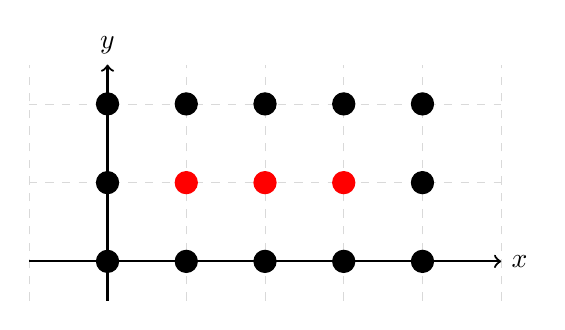
\begin{tikzpicture}
				\draw[help lines, color=gray!30, dashed] (-1,-0.5) grid (5,2.5);
				\draw[->, thick] (-1,0)--(5,0) node[right]{$x$};
				\draw[->, thick] (0,-0.5)--(0,2.5) node[above]{$y$};
				\filldraw[black] (0,0) circle (4pt) node[] {};
				\filldraw[black] (1,0) circle (4pt) node[] {};
				\filldraw[black] (2,0) circle (4pt) node[] {};
				\filldraw[black] (3,0) circle (4pt) node[] {};
				\filldraw[black] (4,0) circle (4pt) node[] {};
				
				\filldraw[black] (0,2) circle (4pt) node[] {};
				\filldraw[black] (1,2) circle (4pt) node[] {};
				\filldraw[black] (2,2) circle (4pt) node[] {};
				\filldraw[black] (3,2) circle (4pt) node[] {};
				\filldraw[black] (4,2) circle (4pt) node[] {};
				
				\filldraw[black] (0,1) circle (4pt) node[] {};
				\filldraw[red] (1,1) circle (4pt) node[] {};
				\filldraw[red] (2,1) circle (4pt) node[] {};
				\filldraw[red] (3,1) circle (4pt) node[] {};
				\filldraw[black] (4,1) circle (4pt) node[] {};
				\end{tikzpicture}	
			\end{figure}
		
		\subsubsection{Laplace Equation}
			This can be used to describe the stead-state of (for example) the heat distribution on a surface:
			\begin{align}
			\partial_{xx} u + \partial_{yy} u &= 0 \\
			\Delta u &= 0 \\
			\nabla^2 u &= 0 
			\end{align}
			
			If the RHS of these equations is a function, $f(x,y)$ we get the \textbf{Poisson Equation}. This is an import equation to solve and comes up in a number of areas (e.g solving pressure fields in computational fluid dynamics). So how do we solve this using the \textit{finite difference method}? Therefore, we wish to solve:
			\begin{align}
			\nabla^2 u = f(x,y)
			\end{align}
			Subject to Dirichlet (fixed value of $u$) and Neumann (fixed derivative of $u$) boundary conditions. Here we can think of the Neumann B.C. as a flux into our system. For simplicity, let us take $\Delta x = \Delta y = h$, than the discrete equation will become:
			\begin{align}
			u_{i+1,j} + u_{i-1,j} + u_{i,j+1} + u_{i,j-1} - 4u_{i,j} - h^2 f_{i,j} = 0 \label{eqn:laplaceDiscrete}
			\end{align}
			
			Therefore, we can do a similar domain deconstruction as with the wave equation and write algebraic expressions for each unknown grid point.
	\section{Week 11}
		\subsubsection{Laplace / Poisson's Equation Continued... Iterative solution methods!}
			For this, we are going to look at three methods of solving our system of unknowns created when we write out the discrete form of the Laplace/Poisson equations for each node in our discrete domain:
			\begin{enumerate}
				\item Jacobi method;
				\item Gauss-Seidel method;
				\item Successive over-relaxation method.
			\end{enumerate}
		
		\subsubsection{Jacobi's Method}
			This is perhaps the simplest method for solving systems such as, $A\mathbf{x} = b$, and gives a good basis for understanding more complex iterative schemes. In the past this method has not been overly used for practical solutions, however, with the advent of parallel programming - this is being reconsidered. To apply this scheme, we rearrange Equation \ref{eqn:laplaceDiscrete} to obtain,
			\begin{align}
				u_{i,j} &= \frac{1}{4} \left( u_{i+1,j} + u_{i-1,j} + u_{i,j+1} + u_{i,j-1} - h^2 f_{i,j} \right).
			\end{align}
			From here, we make an initial guess, $u_{i,j}^0$ and use this equation to update successive values of $u_{i,j}$ until we converge,
			\begin{align}
				u_{i,j}^{(n+1)} &= \frac{1}{4} \left( u_{i+1,j}^{(n)} + u_{i-1,j}^{(n)} + u_{i,j+1}^{(n)} + u_{i,j-1}^{(n)} - h^2 f_{i,j} \right).
			\end{align}
			The good thing about this method, is that it always converges, however, the convergence can be very slow.
			
		\subsubsection{Gauss-Seidel Method}
			This method is a small variation on Jacobi's method in which, once we have calculated $u_{i,j}^{(n+1)}$, why not use it for the next point that we calculate? Namely, if we look at a point located at $(i,j)=(2,2)$, we have most likely already updated $u_{1,2}^{(n+1)}$ and $u_{2,1}^{(n+1)}$:
			\begin{align}
				u_{2,2}^{(n+1)} &= \frac{1}{4} \left( u_{3,2}^{(n)} + u_{1,2}^{(n+1)} + u_{2,3}^{(n)} + u_{2,1}^{(n+1)} - h^2 f_{2,2} \right).
			\end{align}
			
		\subsubsection{Successive Over-Relaxation (SoR) Method}
			Here we look to use a weighted average of the new and old values in our solution such that the previous example would become,
			\begin{align}
				u_{2,2}^{(n+1)} &= (1-\omega)u_{2,2}^{(n)} + \frac{\omega}{4} \left( u_{3,2}^{(n)} + u_{1,2}^{(n+1)} + u_{2,3}^{(n)} + u_{2,1}^{(n+1)} - h^2 f_{2,2} \right).
			\end{align}
			For this, we have,
			\begin{align*}
				\begin{cases}
					\omega < 1, \quad& \text{under-relaxation} \implies \text{slows down convergence} \\
					\omega = 1, \quad& \text{Gauss-Seidel} \\
					\omega > 1, \quad& \text{over-relaxation}  \implies \text{speeds up convergence}
				\end{cases}
			\end{align*}
			
		\textit{Aside:} if we have flux boundary conditions, we can use the second order, three-part approximation,
		\begin{align}
			f'(x) = \frac{-3f(x) + 4f(x+h) - f(x+2h)}{2h} + O(h^2)
		\end{align}
		
		\subsection{Interpolation}
			The aim we have with interpolation for this section is to find a function that passes through a given data set. This allows us to determine values between data points as well as find lines of best fit. \\
			\textit{Definition:} 
			\begin{center}
			A function, $y=f(x)$, interpolates data points, $(x_i,y_i)$, with $1\leq i \leq n$ if $f(x_i) = y_i$ $\forall i$.
			\end{center}
		
			Here, we will discuss two methods of interpolation,
			\begin{enumerate}
				\item Polynomials: \\
					This is useful as it gives us `straight forward' mathematical properties and allows us to evaluate complicated functions with elementary operators.
					\begin{itemize}
						\item Lagrangian Interpolation \\
						Given $n$ data points $(x_1,y_1),\dots,(x_n,y_n)$, we can define a polynomial that interpolates this,
						\begin{align}
							P(x) &= \sum_{i=1}^n y_i L_i(x), \quad \text{where} \\
							&L_i(x) = \frac{(x-x_1)\dots(x-x_{i-1})(x-x_{i+1})\dots (x-x_n)}{(x_i-x_1)\dots(x_i-x_{i-1})(x_i-x_{i+1})\dots (x_i-x_n)} \nonumber
						\end{align}
						\item Newton's Divided Differences \\
						Let $(x_i,y_i)$ where $i=1,\dots,n$ be $n$ data points with distinct $x_i$. There exists one and only one polynomial, $P$, of degree at most $(n-1)$ such that $P(x_i)=y_i$. For this, we can define the first divided difference,
						\begin{align}
							f[x_0,x_1] = \frac{f(x_1) - f(x_0)}{x_1-x_0},
						\end{align}
						and the second divided diffence as,
						\begin{align}
							f[x_0, x_1,x_2] = \frac{f[x_1,x_2]-f[x_0,x_1]}{x_2-x_0}.
						\end{align}
						From this, we can define the polynomial that fits the data points as,
						\begin{align}
							f(x) = f(x_0) &+ f[x_0,x_1] + (x-x_0)(x-x_1)f[x_0,x_1,x_2] + \dots \\ 
										  &+ (x-x_0)(x-x_1)\dots(x-x_k) f[x_0,x_1,\dots,x_k]
						\end{align}
						
					\end{itemize}
			\end{enumerate}
		
		\section{Week 12}
		\begin{itemize}
			\item Chebyshev Theorem \\
				Given $n$ data points on the interval $\left[ a,b\right]$, the interpolation error is minimised if $n$ data points are moved to Chebyshev's points (roots),
				\begin{align}
					x_i = \frac{b-a}{2} \cos \left(\frac{(2i-1)\pi}{2n} \right) + \frac{b+a}{2}, \quad \quad i=1,\dots,n.
				\end{align}
				This way (moving data points) the numerator error is minimised a determinable upper bound,
				\begin{align}
					(x-x_1)(x-x_2)\dots(x-x_n) \leq \frac{(b-a)^n}{2^{2n-1}}.
				\end{align}
		\end{itemize}
		\begin{enumerate}
			\setcounter{enumi}{1}
			\item Splines \\
				In polynomial interpolation we used a single polynomial to interpolate between all data points. With splines, we now use up to $(n-1)$ polynomials to interpolate $n$ points. Here, it is common practice to use cubic polynomials, which is sufficient to satisfy;
				\begin{itemize}
					\item spline is continuous;
					\item spline is smooth;
					\item spline has some curvature.
				\end{itemize}
			For a \textit{natural spline}, we also have the condition that $s_1''(x_1)=s''_{n-1}(x_{n-1})=0$. \\
			
			From all of these conditions, we end up with $3(n-1)$ equations and $3(n-1)$ unknowns. Namely, we have $(n-1)$ points and three coefficients at each to calculate. Therefore, we take our approximation,
			\begin{align}
				s_i(x) = a_i + b_i(x-x_i) + c_i(x-x_i)^2 + d_i(x-x_i)^3, \qquad a_i = y_i,
			\end{align}
			and seek to determine $b_i,c_i,d_i$. This is done by taking,
			\begin{align}
				\delta_i &= x_{i+1} - x_i \\
				\Delta_i &= y_{i+1} - y_i,
			\end{align}
			such that we can define $b,d$ in terms of $c$ as,
			\begin{align}
				d_i &= \frac{c_{i+1}-c_i}{3*J_i},\\
				b_i &= \frac{\Delta_i}{\delta_i} - \frac{\delta_i}{3} (2c_i+c_{i+1}).
			\end{align}
			To solve for $c_i$, the equations from the above spline conditions allow us to write,
			\begin{align}
			\begin{pmatrix}
				1 		 & 	0 						& 	0 			& \dots & \dots \\
				\delta_1 &	2(\delta_1+\delta_2)	&	\delta_2	& 0		& \dots \\
				0		 &	\delta_2		& 2(\delta_2+\delta_3)	& \delta_3 & \dots \\
				\vdots	 &	\ddots			& \ddots				&\ddots	& \ddots \\
				0		 & 0				& 0						& 0		& 1
			\end{pmatrix} \begin{pmatrix}
			c_1 \\ c_2 \\ \vdots \\ \vdots \\ c_n
			\end{pmatrix} = 
			\begin{pmatrix}
			0 \\ 3 (\Delta_2/\delta_2 - \Delta_1/\delta_1) \\ \vdots \\ 3 (\Delta_{n-1}/\delta_{n-1} - \Delta_{n-2}/\delta_{n-2}) \\ 0
			\end{pmatrix}
			\end{align}
		\end{enumerate}
	
		\subsection{Extrapolation}
			Rather than interpolating within the range of data we have, we will now look at methods for extrapolating beyond our given range.
			\subsubsection{Richardson's Extrapolation Method}
				Here the idea is to use multiple step sizes to improve the approximation,
				\begin{align}
					v_t&\approx v_a(h) + kh^n \\
					v_t&\approx v_a(h/2) + k (h/2)^n \\
					\implies &v_t(1-2^n) \approx v_a(h)-2^n v_a(h/2),
				\end{align}
				therefore, our extrapolated approximation becomes,
				\begin{align}
					v_t \approx v_a(h/2) + \frac{v_a (h/2) - v_a(h)}{2^n-1}.
				\end{align}
		\subsection{Numerical Integration}
		\begin{enumerate}
			\item Newton-Cotes formulas, estimate integration with equally spaced points
			\begin{enumerate}
				\item Trapezoidal rule
				\item Simpson's rule
				\item Romberg rule (extrapolation.)
			\end{enumerate}
			\item Adaptive quadrature \\
			Numerical integration is based on evaluating integral by adapting size of intervals. 
		\end{enumerate}
\end{document}
